\section{Simplification of Navier-Stokes}

% ===== Slide 1 =====
\begin{secframe}
\small
\textcolor{red_unipd}{\Large Navier--Stokes (2D, incompressible)}

\vspace{0.6em}

\begin{alertblock}{Equation}
\[
\begin{cases}
\dfrac{\partial \mathbf{u}}{\partial t} 
+ (\mathbf{u}\!\cdot\!\nabla)\mathbf{u}
= -\nabla p + \nu\nabla^2 \mathbf{u},\\[4pt]
\nabla\!\cdot\!\mathbf{u} = 0
\end{cases}
\]
\end{alertblock}

\begin{block}{Hypotheses}
Incompressible: \(\nabla\!\cdot\!\mathbf{u} = 0\). \quad
Viscous: \(\nu>0\). \quad
Free pressure: \(p(x,y,t)\).
\end{block}

\vspace{0.5em}
\textit{Used in:}  
– PINN (Raissi et al., 2017)  
– FNO (Li et al., 2020)  
– NFTM (Malhotra \& Seghouani, 2025)  
– PDEBench: compressible \& incompressible Navier–Stokes datasets
\end{secframe}


% ===== Slide 2 =====
\begin{secframe}
\small
\textcolor{red_unipd}{\Large Euler (Inviscid Fluid)}

\vspace{0.6em}

\begin{alertblock}{Equation}
\[
\dfrac{\partial \mathbf{u}}{\partial t} 
+ (\mathbf{u}\!\cdot\!\nabla)\mathbf{u}
= -\nabla p
\]
\end{alertblock}

\begin{block}{Hypotheses}
No viscosity: \(\nu = 0\). \quad
(Optional) Incompressible: \(\nabla\!\cdot\!\mathbf{u}=0\).
\end{block}

\vspace{0.5em}
\textit{Used in:}  
– Mentioned in NFTM discussions (Malhotra, 2025)  
– Not directly used in PINN/FNO/PDEBench (unstable formulation)
\end{secframe}


% ===== Slide 3 =====
\begin{secframe}
\small
\textcolor{red_unipd}{\Large Burgers (1D Advection–Diffusion)}

\vspace{0.6em}

\begin{alertblock}{Equation}
\[
\dfrac{\partial u}{\partial t} + u\dfrac{\partial u}{\partial x}
= \nu\dfrac{\partial^2 u}{\partial x^2}
\]
\end{alertblock}

\begin{block}{Hypotheses}
\(\nabla p=\mathbf{0}\). \quad
1D reduction: \(\mathbf{u}=(u(x,t),0)\). \quad
Self-advection: \(u\,\partial_x u\).
\end{block}

\vspace{0.5em}
\textit{Used in:}  
– PINN (Raissi et al., 2017) — canonical nonlinear PDE example  
– FNO (Li et al., 2020) — 1D Burgers dataset (autoregressive rollout)  
– NFTM — simplified dynamic for iterative refinement  
– PDEBench \& NeuralOperator Burgers datasets
\end{secframe}


% ===== Slide 4 =====
\begin{secframe}
\small
\textcolor{red_unipd}{\Large Heat / Diffusion Equation}

\vspace{0.6em}

\begin{alertblock}{Equation}
\[
\dfrac{\partial u}{\partial t} =
\alpha\,\dfrac{\partial^2 u}{\partial x^2}
\]
\end{alertblock}

\begin{block}{Hypotheses}
No convection: \(u\,\partial_x u = 0\). \quad
Pure diffusion: \(\alpha>0\).
\end{block}

\vspace{0.5em}
\textit{Used in:}  
– NFTM GitHub repository (“heat equation” baseline)  
– PDEBench diffusion/heat datasets  
– Used to test backtracking, teacher forcing, and refinement stability
\end{secframe}


% ===== Slide 5 =====
\begin{secframe}
\small
\textcolor{red_unipd}{\Large Darcy (Steady, Elliptic Form)}

\vspace{0.6em}

\begin{alertblock}{Equation}
\[
\nabla\!\cdot\!\big(a(x)\nabla u(x)\big) = f(x)
\]
\end{alertblock}

\begin{block}{Hypotheses}
Steady regime: \(\partial_t u = 0\). \quad
Heterogeneous medium: \(a(x)>0\). \quad
Source/sink: \(f(x)\).
\end{block}

\vspace{0.5em}
\textit{Used in:}  
– PINN (Raissi et al., 2017) — steady-state diffusion problem  
– FNO (Li et al., 2020) — 2D Darcy dataset in NeuralOperator  
– PDEBench Darcy flow benchmark  
– Tested under hybrid and data-driven regimes
\end{secframe}


\begin{secframe}
\small
\textcolor{red_unipd}{\Large Simplification Path of Fluid Dynamics Equations}

\medskip
\centering
\resizebox{.95\linewidth}{!}{%
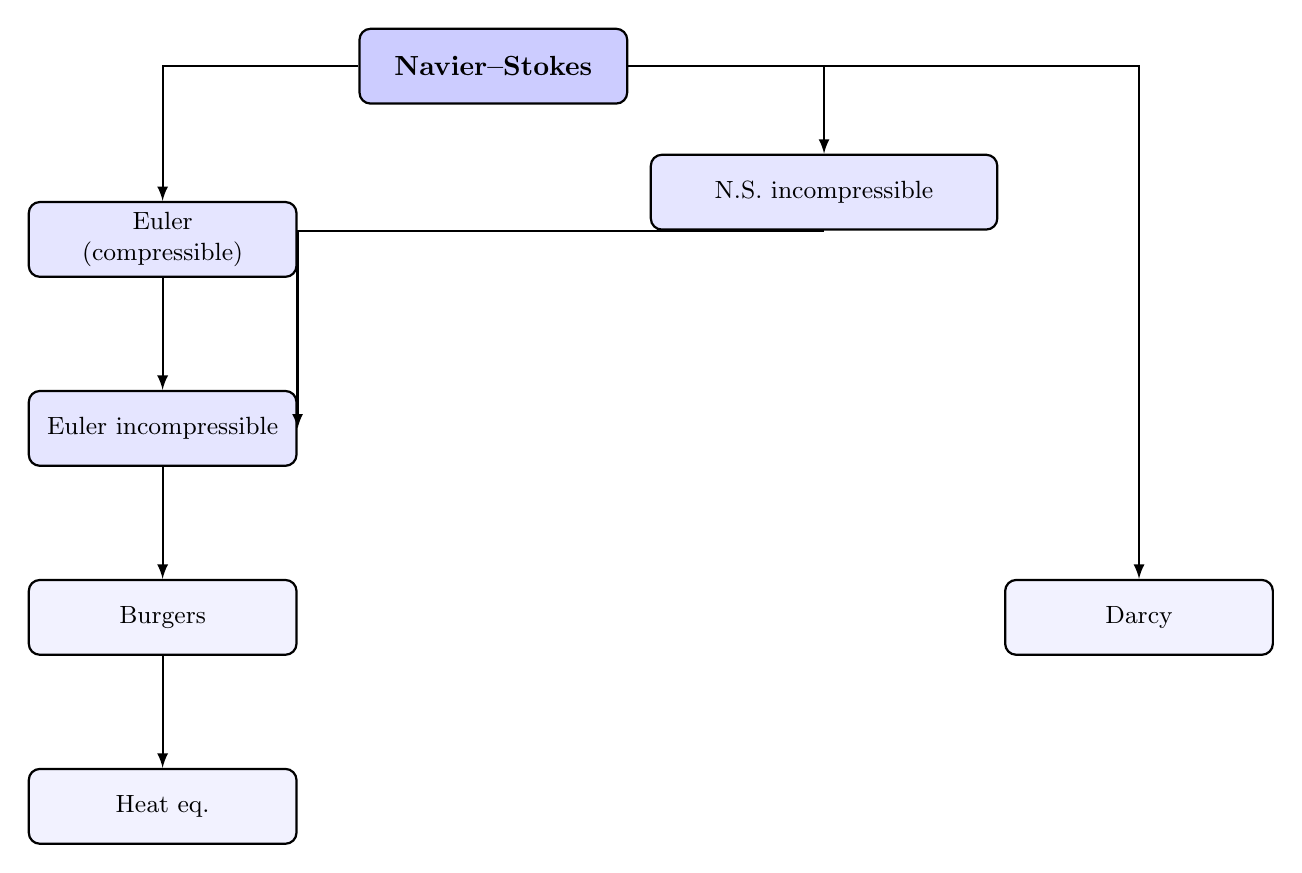
\begin{tikzpicture}[
  >=latex,
  box/.style={draw,rounded corners,thick,minimum width=3.4cm,minimum height=0.95cm,align=center},
  every node/.style={font=\small}
]
% --- Nodes ---
\node[box,fill=blue!20,font=\bfseries] (NS) at (0,0) {Navier--Stokes};

% left vertical chain
\node[box,fill=blue!10] (E)   at (-4.2,-2.2) {Euler\\(compressible)};
\node[box,fill=blue!10] (EI)  at (-4.2,-4.6) {Euler incompressible};
\node[box,fill=blue!5]  (B)   at (-4.2,-7.0) {Burgers};
\node[box,fill=blue!5]  (H)   at (-4.2,-9.4) {Heat eq.};

% right branch
\node[box,fill=blue!10,minimum width=4.4cm] (NSi) at (4.2,-1.6) {N.S.\ incompressible};
\node[box,fill=blue!5] (D)    at (8.2,-7.0) {Darcy};

% --- Arrows: H then V only ---
% NS -> Euler
\draw[->,thick] (NS.west) -- (E.north |- NS.west) -- (E.north);
% Euler vertical chain
\draw[->,thick] (E)  -- (EI);
\draw[->,thick] (EI) -- (B);
\draw[->,thick] (B)  -- (H);
% NS -> N.S. incompressible
\draw[->,thick] (NS.east) -- (NSi.north |- NS.east) -- (NSi.north);
% N.S. incompressible -> Euler incompressible
\draw[->,thick] (NSi.south) -- (EI.east |- NSi.south) -- (EI.east);
% NS -> Darcy
\draw[->,thick] (NS.east) -- (D.north |- NS.east) -- (D.north);

\end{tikzpicture}%
}
\end{secframe}






